\documentclass{article}\usepackage[]{graphicx}\usepackage[]{xcolor}
% maxwidth is the original width if it is less than linewidth
% otherwise use linewidth (to make sure the graphics do not exceed the margin)
\makeatletter
\def\maxwidth{ %
  \ifdim\Gin@nat@width>\linewidth
    \linewidth
  \else
    \Gin@nat@width
  \fi
}
\makeatother

\definecolor{fgcolor}{rgb}{0.345, 0.345, 0.345}
\newcommand{\hlnum}[1]{\textcolor[rgb]{0.686,0.059,0.569}{#1}}%
\newcommand{\hlsng}[1]{\textcolor[rgb]{0.192,0.494,0.8}{#1}}%
\newcommand{\hlcom}[1]{\textcolor[rgb]{0.678,0.584,0.686}{\textit{#1}}}%
\newcommand{\hlopt}[1]{\textcolor[rgb]{0,0,0}{#1}}%
\newcommand{\hldef}[1]{\textcolor[rgb]{0.345,0.345,0.345}{#1}}%
\newcommand{\hlkwa}[1]{\textcolor[rgb]{0.161,0.373,0.58}{\textbf{#1}}}%
\newcommand{\hlkwb}[1]{\textcolor[rgb]{0.69,0.353,0.396}{#1}}%
\newcommand{\hlkwc}[1]{\textcolor[rgb]{0.333,0.667,0.333}{#1}}%
\newcommand{\hlkwd}[1]{\textcolor[rgb]{0.737,0.353,0.396}{\textbf{#1}}}%
\let\hlipl\hlkwb

\usepackage{framed}
\makeatletter
\newenvironment{kframe}{%
 \def\at@end@of@kframe{}%
 \ifinner\ifhmode%
  \def\at@end@of@kframe{\end{minipage}}%
  \begin{minipage}{\columnwidth}%
 \fi\fi%
 \def\FrameCommand##1{\hskip\@totalleftmargin \hskip-\fboxsep
 \colorbox{shadecolor}{##1}\hskip-\fboxsep
     % There is no \\@totalrightmargin, so:
     \hskip-\linewidth \hskip-\@totalleftmargin \hskip\columnwidth}%
 \MakeFramed {\advance\hsize-\width
   \@totalleftmargin\z@ \linewidth\hsize
   \@setminipage}}%
 {\par\unskip\endMakeFramed%
 \at@end@of@kframe}
\makeatother

\definecolor{shadecolor}{rgb}{.97, .97, .97}
\definecolor{messagecolor}{rgb}{0, 0, 0}
\definecolor{warningcolor}{rgb}{1, 0, 1}
\definecolor{errorcolor}{rgb}{1, 0, 0}
\newenvironment{knitrout}{}{} % an empty environment to be redefined in TeX

\usepackage{alltt}
\usepackage{amsmath} %This allows me to use the align functionality.
                     %If you find yourself trying to replicate
                     %something you found online, ensure you're
                     %loading the necessary packages!
\usepackage{amsfonts}%Math font
\usepackage{graphicx}%For including graphics
\usepackage{hyperref}%For Hyperlinks
\usepackage[shortlabels]{enumitem}% For enumerated lists with labels specified
                                  % We had to run tlmgr_install("enumitem") in R
\hypersetup{colorlinks = true,citecolor=black} %set citations to have black (not green) color
\usepackage{natbib}        %For the bibliography
\setlength{\bibsep}{0pt plus 0.3ex}
\bibliographystyle{apalike}%For the bibliography
\usepackage[margin=0.50in]{geometry}
\usepackage{float}
\usepackage{multicol}

%fix for figures
\usepackage{caption}
\newenvironment{Figure}
  {\par\medskip\noindent\minipage{\linewidth}}
  {\endminipage\par\medskip}
\IfFileExists{upquote.sty}{\usepackage{upquote}}{}
\begin{document}

\vspace{-1in}
\title{Lab 02 -- MATH 240 -- Computational Statistics}

\author{
  Jack Schaeffer \\
  Professor Cipolli \\
  MATH 240 \\
  {\tt jschaeffer@colgate.edu}
}

\date{}

\maketitle

\begin{multicols}{2}
\begin{abstract}
This lab focused on using \texttt{R} code to procure data about various songs for analysis. Additionally, the lab focused on skills producing plots and tables to assist with interpretation.
\end{abstract}

\noindent \textbf{Keywords:} Lists; Objects in R, Coding Structures, Graphs, Tables

\section{Introduction}
This lab is focused on the song Allentown, a song released by The Front Bottoms and Manchester Orchestra (and also with additional writing credit to All Get Out). The main question of the lab is determining which artist had the greatest influence on Allentown. To do so, several data processing tools were used. These include Essentia for song analysis and a language analysis tool called LIWC, which utilized \texttt{jsonlite} to manipulate the data in \texttt{R} \citep{essentia} \citep{jsonlite}.In the rest of this report, I will explain how these tools produced helpful data and how this data was analyzed to obtain a proposed answer to what artist most influenced Allentown.

\section{Methods}

A majority of the work that went into the lab was focused on acquiring data for future analysis of each artist and the song Allentown. The package \texttt{stringr} was very helpful for taking our song files and prepping them for data extraction \citep{stringr}. The data was then collected through JSON files loaded by \texttt{jsonlite} as well as Essentia \citep{jsonlite} \citep{essentia}. The last set of information included lyrical analysis through LIWC. Once the data was collected, information on Allentown was compared to each song written by the three specified artists to determine what parameters were out of the standard range of each artist. \texttt{xtable} and \texttt{ggplot} were used to form the table and plot featured below for analysis. These were the main resources used to make interpretations on what artist had the greatest influence on Allentown \citep{xtable} \citep{ggplot2}.

\section{Results}
The initial result from our lab was an extensive list of information that would be extremely difficult to analyze as it consisted of over 100 different qualities and their values for each song. Using a summary of information for each artist, the code produced results for Allentown and whether it remained within the bounds of each artist for various features. The data was counted and produced the following table detailing the number of times Allentown exhibited qualities that were outside the bounds of each artist.




% latex table generated in R 4.4.2 by xtable 1.8-4 package
% Tue Feb 25 13:09:48 2025
\begin{table}[H]
\centering
\begingroup\small
\begin{tabular}{llr}
  \hline
Artist & Description & Count \\ 
  \hline
All Get Out & Out of Range &  22 \\ 
  All Get Out & Outlying &  17 \\ 
  All Get Out & Within Range & 158 \\ 
  Manchester Orchestra & Out of Range &   3 \\ 
  Manchester Orchestra & Outlying &  11 \\ 
  Manchester Orchestra & Within Range & 183 \\ 
  The Front Bottoms & Out of Range &  30 \\ 
  The Front Bottoms & Outlying &  11 \\ 
  The Front Bottoms & Within Range & 156 \\ 
   \hline
\end{tabular}
\endgroup
\caption{Count of Allentown in Comparison to Each Artist} 
\label{count.tab}
\end{table}


The results provide helpful information to compare Allentown to the other artists. Unlike the more complicated information, this table provides a far more understandable group of information that shows that Allentown tends to align more closely to certain artists. An even better way to compare the values of each artist can be done with the following plot:

\begin{figure}[H]
 \begin{center}
 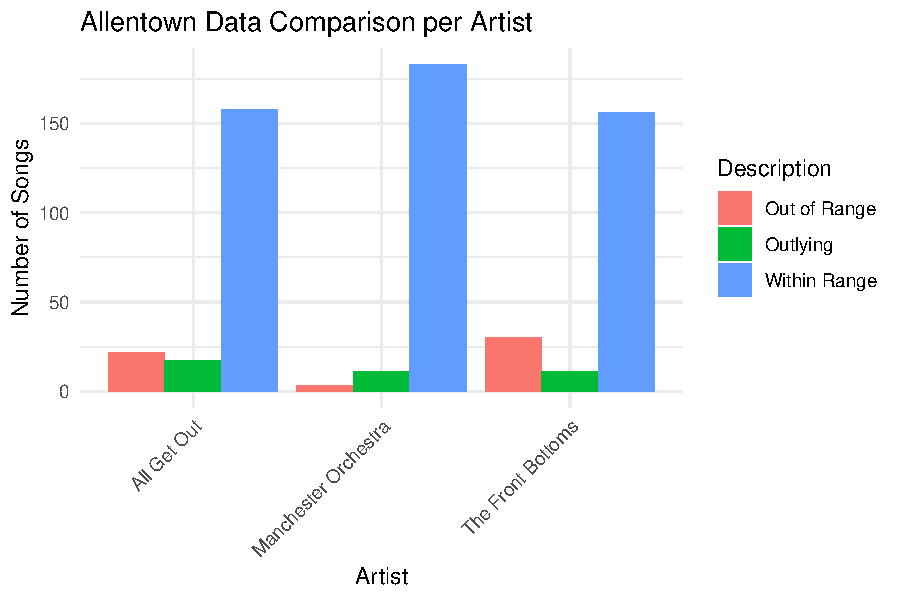
\includegraphics[scale=0.65]{descript_plot.pdf}
 \caption{A comparison of Allentown's data to each artist}
 \label{plot3}
 \end{center}
 \end{figure}

This plot shows important comparison among each artist. Values within range, specified in blue, generally demonstrates ways that Allentown is similar to that artist. Values for outlying and out of range shows how Allentown is different from that artist, potentially signifying ways that it was influenced less by that artist.

\section{Discussion}
From the results we acquired during the lab, it would seem that Allentown aligns closely with each of the three artist but has the most similarities to Manchester Orchestra's music. For most features, Allentown is within the standard range of each of the three artists, but there are significant fewer features that are outlying or out of range compared to Manchester Orchestra. It is understandable that All Get Out would not bear the largest similarity as they were not a performing artist for Allentown. This answers the question that Manchester Orchestra had the largest influence on the creation of Allentown. 

An interesting finding from the data, however, is how closely Allentown related to each of the three artists. Due to the nature of song variety, it would be interesting to see if this trend is present in most artists, not just those that contributed to the song. This shows that Allentown was closely related to all three of its contributing artists, and they combined their styles together in a way that ensured Allentown was a blend of all three bands. 

%%%%%%%%%%%%%%%%%%%%%%%%%%%%%%%%%%%%%%%%%%%%%%%%%%%%%%%%%%%%%%%%%%%%%%%%%%%%%%%%
% Bibliography
%%%%%%%%%%%%%%%%%%%%%%%%%%%%%%%%%%%%%%%%%%%%%%%%%%%%%%%%%%%%%%%%%%%%%%%%%%%%%%%%
\vspace{2em}


\begin{tiny}
\bibliography{bib}
\end{tiny}
\end{multicols}

%%%%%%%%%%%%%%%%%%%%%%%%%%%%%%%%%%%%%%%%%%%%%%%%%%%%%%%%%%%%%%%%%%%%%%%%%%%%%%%%
% Appendix
%%%%%%%%%%%%%%%%%%%%%%%%%%%%%%%%%%%%%%%%%%%%%%%%%%%%%%%%%%%%%%%%%%%%%%%%%%%%%%%%


\end{document}
